%%%%%%%%%%%%%%%%%%%%%%%%%%%%%%%%%%%%%%%%%%%%%%%%%%%%%%%%%%%%%%%%%%
%%%%%%%% ICML 2014 EXAMPLE LATEX SUBMISSION FILE %%%%%%%%%%%%%%%%%
%%%%%%%%%%%%%%%%%%%%%%%%%%%%%%%%%%%%%%%%%%%%%%%%%%%%%%%%%%%%%%%%%%

% Use the following line _only_ if you're still using LaTeX 2.09.
%\documentstyle[icml2014,epsf,natbib]{article}
% If you rely on Latex2e packages, like most moden people use this:
\documentclass{article}

% use Times
\usepackage{times}
% For figures
\usepackage{graphicx} % more modern
\usepackage{booktabs}
%\usepackage{epsfig} % less modern
\usepackage{subfigure}

% For citations
\usepackage{natbib}

% For algorithms
\usepackage{algorithm}
\usepackage{algorithmic}

% As of 2011, we use the hyperref package to produce hyperlinks in the
% resulting PDF.  If this breaks your system, please commend out the
% following usepackage line and replace \usepackage{icml2014} with
% \usepackage[nohyperref]{icml2014} above.
\usepackage{hyperref}

% Packages hyperref and algorithmic misbehave sometimes.  We can fix
% this with the following command.
\newcommand{\theHalgorithm}{\arabic{algorithm}}

% Employ the following version of the ``usepackage'' statement for
% submitting the draft version of the paper for review.  This will set
% the note in the first column to ``Under review.  Do not distribute.''
\usepackage{icml2014}


% The \icmltitle you define below is probably too long as a header.
% Therefore, a short form for the running title is supplied here:
\icmltitlerunning{O'Meara, Stephani, Hand}

\begin{document}

\twocolumn[
\icmltitle{Project Report for CIS 419/519\\Stock Recommendations using Machine Learning}

% It is OKAY to include author information, even for blind
% submissions: the style file will automatically remove it for you
% unless you've provided the [accepted] option to the icml2014
% package.
\icmlauthor{Michael O'Meara}{momeara@seas.upenn.edu}
\icmlauthor{Timmy Stephani}{stephan6@seas.upenn.edu}
\icmlauthor{Dave Hand}{handd@seas.upenn.edu}

% You may provide any keywords that you
% find helpful for describing your paper; these are used to populate
% the "keywords" metadata in the PDF but will not be shown in the document
\icmlkeywords{machine learning, stocks, comparison, naive bayes, svm, neural networks}

\vskip 0.3in
]

\begin{abstract}
In this report, we present a simplified stock recommendation system. This system is based on patterns found from the price history of a list of equities. In developing the system, various machine learning techniques were tested to try to predict which stocks should be bought or sold to maximize the percent return going forward. We chose to use naive bayes, neural networks, and a support vector machines with a gaussian kernel as our main machine learning techniques. We trained each model on past data through a backtesting module and then presented each model with new data in order to make predictions. In addition, we utilized our module to test several different combinations of features and compared the accuracy, precision, recall, and percent return of various models.
\end{abstract}

\section{Introduction}
Many financial institutions and investors are wary of trading in the stock market since the financial collapse in 2008.  Almost all financial institutions have turned to machine learning or other algorithmic techniques in order to reduce the risk in trading. Our system is targeted as a longer-term trade recommendation system, avoiding the real-time constraints of high-frequency algorithms. We attempt to solve a small subset of this larger financial landscape, making good short-term predictions for buying or selling stocks that the average investor might be able to utilize.

The principle of our trading strategy is based on the idea that price movements in a stock form technical patterns that represent the sentiment of a particular equity over time. These patterns can help predict the future price movement of a stock, which if known, can improve the overall return for an investor.

\subsection{Model assumptions}
In our implementation, we make several assumptions to simplify the constraints. We believe that while these assumptions necessarily make the algorithms we develop less applicable to the real world, they still remain close to reality. We believe that some of our models could potentially be used by individuals in the real world at some rate of success, but at their own risk. We first assume that the trader has stock in whichever stocks our model was trained on. This allows us to to predict whether to buy, sell, or hold regardless of whether or not the individual actually owns any stock at that current point in time. Our model can be viewed as the global prediction of whether to buy, sell, or hold on a certain day and is not related or tied to any specific trader portfolio.

An additional assumption will be that the closing price reflects the sentiment of that day's price action enough to be considered the price for the entire day. This has the added benefit of avoiding intraday fluctuations in the stock market. We will also ignore all transaction fees and taxes associated with trading on the stock market and simply use a flat fee of 0.5\%.

\subsection{Definition}
In addition to baseline metrics, we added an additional metric for evaluating our models, percent return. This was calculated so that we could compare it to the actual return of the stock over the same period of time. That way, we could empirically see that our model was outperforming the average case. The formula for calculating the percent return is:

$$
Percent Return = \frac{(V_{now} - V_{beginning})}{V_{beginning}}
$$

\section{Methodology}

\subsection{Source of data}
The dataset used was downloaded from Wharton Research Data Services (WRDS). The stocks used are the stocks that comprise the Dow30. The Dow30 is an index of stocks developed as a way of tracking U.S. market performance. It is comprised of the current top thirty blue-chip U.S. stocks. For each stock, we pulled several features, including closing price, high, low, and volume. Our research into the field suggested that these features would be the best for prediction. We pulled stock data from January 1, 1983 to December 31, 2013 to give us a window of 30 years. WRDS does not currently store the data we were utilizing for 2014.

The closing price is the price at the end of a particular time period. The daily closing price is the price at the end of a day. The high and low are the spread between what the buyer must pay for a stock (high) and what the seller would receive for a stock (low). The volume is the number of shares that were traded on a given day for a stock.

The features we used could be pulled in different time frames. For instance, we could pull yearly, monthly, or daily records for closing price. However, our research into the field suggested that a daily time frame would be both the best to predict on and the most desired model as well. Most successful papers trained daily models on past flucutations. In addition, predicting on a daily time frame inherently captures monthly and yearly trends, just on a daily level, which is also more applicable to the individuals who would want to use this.

\subsection{Trading strategy}
Each of our models is designed for determining the best decision for a given day. Therefore, we have a choice of three classes (buy, sell, or hold) to assign to each day in our model. Our model assigns its choice based on the threshold of the transaction fee of 0.5\% we assigned above. If the model is expecting a change of more than 0.5\% in the stock for a particular day, the model will choose to buy or sell accordingly (i.e. if the percentage change is positive or negative). Otherwise, it will predict to hold. The decision to hold is because in these cases, the cost to make the trade is greater than the expected return of the transaction. We then compare the model's choice with the actual best decision, which is calculated by using the actual percent change in the same manner, in order to determine if the model's choice was correct. All predictions, including hold, are counted as successful "trades" if they match the actual best decision. The number of successful trades divided by the number of possible successful trades is how we obtain our accuracy. Calculations for precision and recall are related to the number of successful trades as well.

\subsection{Backtesting}
We have written a backtesting module to look at different time frames and feature sets in our historical trades data. The backtesting module also allows us to choose where our time frame begins and ends, i.e. if we only wanted to use the last one-hundred days of 2013 for our training and testing. After researching how backtesting is implemented in real-world environments, we have also implemented pattern recognition in our backtesting code to confirm that there are trends we could exploit.

Some example patterns that our system found are illustrated below with the current pattern in cyan. The other lines are past patterns that our system found that are potential matches and the dots to the right represent outcomes for each past pattern.  The rightmost dots are the actual outcome and average of the past patterns.

\begin{figure}[h!]
\begin{center}
        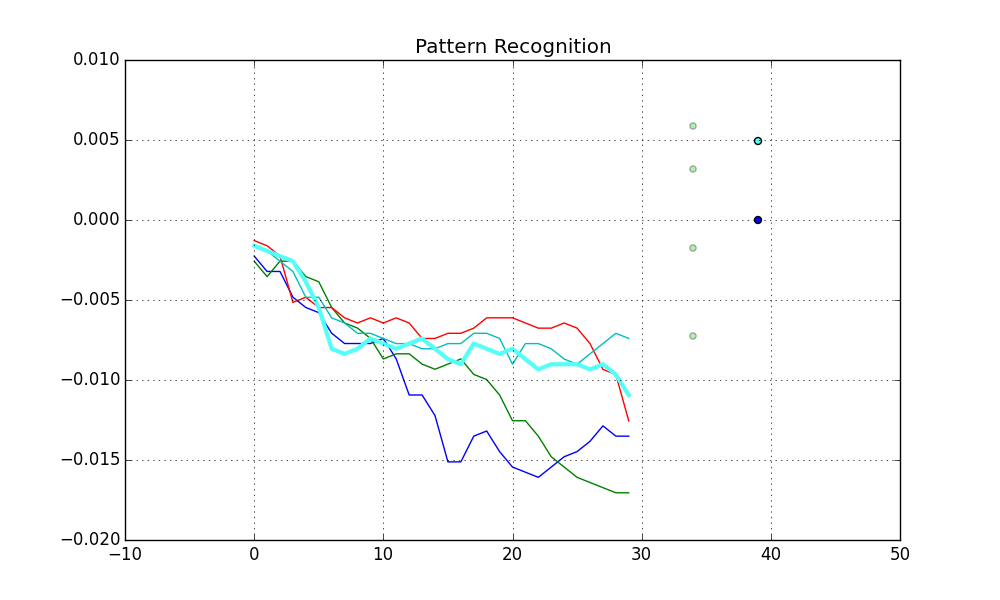
\includegraphics[scale=0.3]{figure_2}
        \caption{Examples of downward trend reversals}
\end{center}
\end{figure}

\begin{figure}[h!]
\begin{center}
        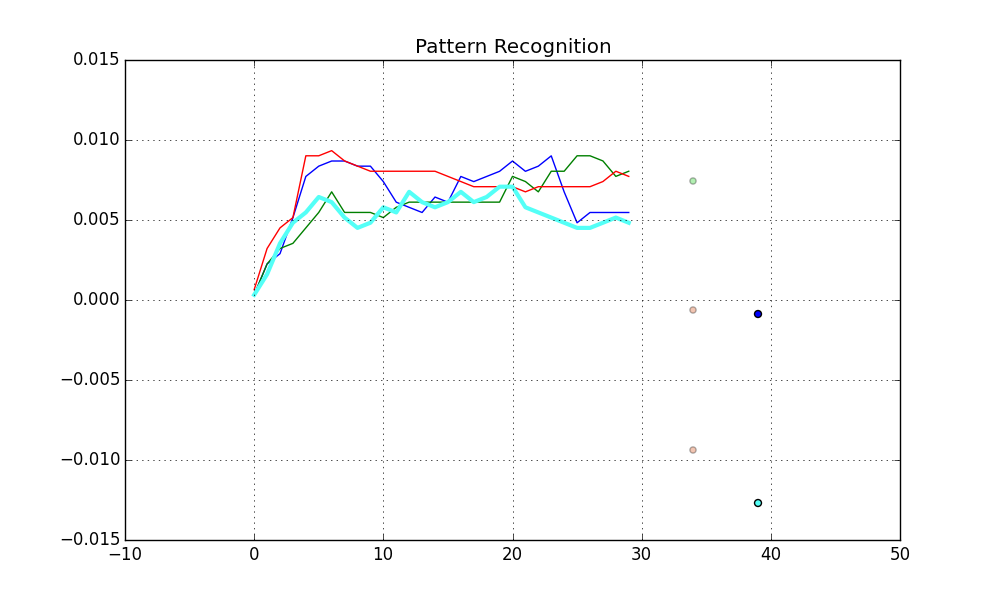
\includegraphics[scale=0.3]{figure_3}
        \caption{Examples of upward trend reversal}
\end{center}
\end{figure}

\subsection{Machine learning framework}
At this point, we've also set up another framework that allows us to easily evaluate different classifiers, different time frames (10 or 100 days), and different features easily. The framework receives the patterns and features from the backtesting module. The framework is designed for handling time-series data and uses a specified number of past days in order to make a trade prediction for a specific day. For instance, if we specified our window to be ten days, the model would have been trained on the past ten days and then utilize that knowledge to predict on the specific day. We then would slide the entire ten day window forward one day and retrain the model in order to predict on the following day. We utilized validation sets in order to find the best features from our dataset. Our framework also utilized grid-search for finding the best-tuned variables for some models. This helped us determine which features, data, and window size to use to train each respective model for the best results.

\subsection{Training and Analysis Overview}
\begin{figure}[h!]
\begin{center}
        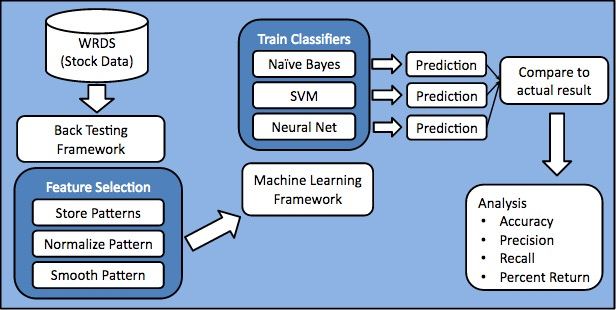
\includegraphics[scale=0.37]{summary_fig}
        \caption{Framework summary}
\end{center}
\end{figure}

Through the framework, we found that each model had the most success when using the closing price as the sole feature. We did not find any statistically significant differences in a model's predictive power when using data from several decades ago as opposed to data from recent years. We also found negligible returns on our metrics after increasing the window past twenty-one days.

We utilized our machine learning framework to train and analyze the performance of each of the following models: naive bayes, SVM with gaussian kernel, and a neural network. Based on our findings in the above paragraphs, we evaluated each model using closing price on the last one-hundred days of 2013. We utilized a twenty-one day window for our analysis of each model.

Our models were evaluated on four specific criteria: accuracy, precision, recall, and the percent return. In addition to those base metrics, we also calculated the percent return as defined above in order to better determine the financial success of our model. For example, our model could predict with a high accuracy, but only on days that produce negligible returns. Therefore, percent return provides a way to verify that our correct predictions are more than just correct, they also need to be profitable. We can determine if our percent return is successful by comparing it with the stock's average actual percent return over the same period. If we outperform the actual average percent return, we consider our model to be successful.

Our main goal for each model was to maximize the percent return over the thirty stocks. If we could outperform the Dow30's average return over the same time frame, then we would have empirical evidence of the success of our model. For reference, the Dow30 percent return on the last one-hundred days of 2013 was 16.31\%.

\section{Model Analysis}

\subsection{Naive Bayes}
The first machine learning classifier we analyzed was naive Bayes. Through research into past papers on the topic, it appeared many people had mixed results when trying to use naive bayes to predict trades. We did not expect naive Bayes to perform well, but we did expect it to produce results better than random guessing. We felt that the probabilistic elements in Naive Bayes would allow it to predict the correct trend for a particular day, which would equate to predicting the correct action for the day.

Unfortunately, we were not able to achieve statistically significant results with our naive Bayes implementation. We averaged around 51.3\% accuracy and a 16.1\% return for the model, which was not able to outperform the averge Dow30 return over the same time frame. In other words, an investor's return would have been better if he/she did nothing instead of following the model's recommendations.

Looking back, we believe that the the reason our model failed to perform better than the average was that the data is intrinsically related and not independent. As successive days were directly correlated with previous days, it was hard for naive Bayes to fit and predict well on the data. In addition, the zero autocorrelation between stock prices helps to explain why naive Bayes may not be the best choice.

As our results for naive Bayes were not empirically good or statistically significant, we are not going to display the results for each individual stock in the Dow30. We will display the data for our two other, more successful models.

\subsection{SVM (gaussian)}
The second machine learning classifier we analyzed was a support vector machine with a gaussian kernel. Research into using support vector machines for predicting stocks had given us insight into how successful these models could be. In addition, gaussian svms could fit our trend data very well and can be very efficient for smaller datasets. The svm would most likely fit to stronger trends as well (with proper tuning), so some of the noise in the data would be well filtered. We expected the svm to perform very well on the data and to provide us with a better percent return on the Dow30 than the average. After tuning the parameters with a lengthy grid search, we found that our optimal svm had very respectable predictive power.

On average over the thirty stocks, our svm model predicted the correct trade with an accuracy of 67.97\%. We also averaged a 34.93\% return over the thirty stocks, meaning that we more than doubled the average percent return over the same time frame. It is important to note that the predictions and percent return are based on a simplified model, without factoring in transaction costs. However, these returns are still much higher than average and could be useful for many traders on the stock market.

The results for each of the Dow30 stocks are displayed to the right in Table 1.

\begin{table}[h!]
  \begin{tabular}{@{}lllllll@{}}
    \toprule
    Ticker & Accuracy & Precision & Recall & \% Return & \\ \midrule
    MCD & 90 & 81 & 90.55 & 48.99 & \\
    XOM & 85 & 72.25 & 86.48 & 48.27 & \\
    KO & 82 & 67.24 & 82.96 & 42.51 & \\
    GE & 74 & 54.76 & 77.43 & 41.33 & \\
    MMM & 79 & 62.41 & 79.82 & 40.95 & \\
    PFE & 76 & 57.76 & 77.56 & 40.48 & \\
    IBM & 72 & 51.84 & 74.52 & 38.91 & \\
    VZ & 62 & 38.44 & 65.66 & 38.44 & \\
    JNJ & 78 & 60.84 & 78.24 & 38.08 & \\
    MRK & 84 & 70.56 & 84.88 & 37.72 & \\
    PG & 73 & 53.29 & 75.28 & 37.48 & \\
    UNH & 64 & 40.96 & 67.96 & 36.74 & \\
    WMT & 83 & 68.89 & 83.74 & 36.73 & \\
    AXP & 64 & 40.96 & 66.26 & 36.05 & \\
    T & 68 & 46.24 & 70.34 & 34.65 & \\
    CAT & 70 & 49 & 74.26 & 34.6 & \\
    V & 59 & 34.81 & 61.74 & 33.8 & \\
    CSCO & 69 & 47.61 & 70.24 & 33.57 & \\
    INTC & 66 & 43.56 & 68.92 & 32.81 & \\
    JPM & 65 & 42.25 & 68.48 & 32.71 & \\
    DD & 70 & 49 & 72.52 & 32.51 & \\
    BA & 53 & 28.09 & 54.24 & 32.16 & \\
    G & 72 & 51.84 & 73.96 & 31.3 & \\
    HD & 67 & 44.9 & 69.68 & 30.08 & \\
    MSFT & 61 & 37.21 & 63.14 & 29.65 & \\
    NKE & 68 & 46.24 & 68.74 & 29.22 & \\
    GS & 56 & 31.36 & 57.54 & 28.28 & \\
    UTX & 63 & 39.69 & 63.88 & 28.25 & \\
    DIS & 59 & 34.81 & 60.23 & 27.64 & \\
    C & 53 & 28.09 & 55.84 & 26.99 & \\
    TRV & 48 & 23.04 & 48.64 & 13.71 & \\ \bottomrule
    Average & 68.80 & 48.35 & 70.77 & 34.66 & \\
  \end{tabular}
  \caption{SVM Results for the Dow30}
  \label{my-label}
\end{table}

The svm illustrates empirical success in predicting the correct trade decision for a simplified stock trading model. It validated our initial assumptions and justifications that the svm would be successful.

\subsection{Neural network}
The final machine learning classifier we analyzed was a neural network. There were some papers we found analyzing neural network performance, but we mainly decided to try it as many quantitative finance teams in industry utilize neural networks in order to make predictions on current market trends. Faced with this knowledge, we expected the neural network to perform well and outperform the Dow30 average percent return.

Our neural network consisted of three hidden layers and adhered to the Baum-Hassler rule. This rule was developed for financial forecasting with neural networks. The formula output that we should utilize three hidden layers. The same paper also suggested the number of nodes for each layer. The two outer hidden layers should have $2*num\_input\_nodes + 1$ nodes and the middle hidden layer should have $2*num\_input\_nodes - 1$ nodes. As we used twenty-one days for our input, the hidden layer sizes were $<43,41,43>$ respectively. Our neural network was trained on one-hundred epochs, as we only saw negligible improvements when increasing the number of epochs (our model was already converging).

On average over the thirty stocks, our neural network performed very well. Our neural network had an average trade prediction accuracy of 68.81\% and an average 34.66\% return. We more than doubled the average return of the Dow30 over the same time period. The results here are slightly more optimistic than they should be, as our model was trained and predicted on a reduced stock model with a fixed transaction costs. However, the model still performs very well and would definitely prove very helpful for traders looking for an edge.

The results for the neural network on all thirty stocks are printed on the following page in Table 2.

\begin{table}[h!]
  \begin{tabular}{@{}lllllll@{}}
    \toprule
    Ticker & Accuracy & Precision & Recall & \% Return & \\ \midrule
    MCD & 90 & 81 & 90.43 & 48.99 & \\
    MMM & 79 & 62.41 & 80.12 & 48.95 & \\
    XOM & 85 & 72.25 & 85.23 & 48.27 & \\
    KO & 82 & 67.24 & 83.45 & 42.5 & \\
    GE & 74 & 54.76 & 76.72 & 41.33 & \\
    PFE & 76 & 57.76 & 77.82 & 40.48 & \\
    IBM & 72 & 51.84 & 73.15 & 38.91 & \\
    VZ & 62 & 38.44 & 64.26 & 38.44 & \\
    JNJ & 78 & 60.84 & 78.98 & 38.09 & \\
    MRK & 84 & 70.56 & 84.84 & 37.72 & \\
    PG & 73 & 53.29 & 75.74 & 37.48 & \\
    UNH & 64 & 40.96 & 67.04 & 36.74 & \\
    WMT & 83 & 68.89 & 83.44 & 36.72 & \\
    AXP & 64 & 40.96 & 65.82 & 36.05 & \\
    INTC & 66 & 62.46 & 66.56 & 35.86 & \\
    CAT & 69 & 48.79 & 70.56 & 34.44 & \\
    T & 67 & 46.02 & 68.78 & 34.18 & \\
    JPM & 65 & 42.68 & 68.34 & 32.71 & \\
    DD & 70 & 49 & 71.66 & 32.51 & \\
    V & 49 & 36.88 & 51.08 & 31.8 & \\
    CSCO & 63 & 49.25 & 63.6 & 31.48 & \\
    G & 72 & 51.48 & 73.48 & 31.3 & \\
    BA & 52 & 28.12 & 52.78 & 31.15 & \\
    MSFT & 61 & 37.21 & 63.21 & 29.65 & \\
    NKE & 68 & 46.24 & 69.78 & 29.22 & \\
    HD & 66 & 44.67 & 67.34 & 29.06 & \\
    GS & 54 & 43.15 & 54.53 & 28.47 & \\
    UTX & 63 & 39.69 & 65.98 & 28.25 & \\
    DIS & 58 & 34.57 & 59.28 & 27.46 & \\
    C & 52 & 27.84 & 55.22 & 26.26 & \\
    TRV & 46 & 45.12 & 46.16 & 18.4 & \\ \bottomrule
    Average & 67.97 & 50.14 & 69.53 & 34.93 & \\
  \end{tabular}
  \caption{Neural Net Results for the Dow30}
  \label{my-label}
\end{table}

The neural net illustrates empirical success in predicting the correct trade decision for a simplified stock trading model. It validated our initial assumptions and justifications that it would be a successful model for our purposes.

\subsection{Overall comparison}
We had a large amount of success with two of the three models we trained, which is exactly what we expected to see. We did not predict that our successful models would perform as well as they did. Both the svm and neural network had a high percent return and accuracy and executed successful buy and hold strategies for most stocks. The svm performed slightly better in terms of percent return, while the neural network had a slightly higher accuracy. Both outperformed the Dow30 average percent return, meaning we can empirically state that our implementations are successful and would be useful for traders looking for an edge.

Determining the better classifier of the two is difficult, as the svm and neural net each slightly outperformed the other in different metrics. If we were to choose, we would select the neural net, as it provides a slightly higher percent return, which is the most important metric in our evaluation. It is also important to note that the svm was much faster to train than the neural net, so the slight tradeoff in efficiency may be worth the time savings for some domains.

The svm and neural net accuracy and percent return do fluctuate quite a bit between some of the stocks, having higher predictive power for some (MRK, MCD) and less for others (TRV, V). Through some deeper digging, this appears to be the result of the svm performing better on more stable stocks (segements such as drugs, food, and retail) when compared to more volatile stocks (segements such as insurance and finance). While it is obvious that stocks that fluctuate more wildly than average may be harder to predict, it is interesting to note that the svm and neural network had the same difficulties.

\section{Future Work}
While we have been very successful in achieving our goals, we believe that there are additional changes we could make in order to produce more successful models. One change we could make is smoothing the data and trends output by the backtesting module. Through smoothing, we could remove a lot of the smaller fluctuations and focus more on the major trends.

Another change we could implement is expanding the sliding window and weighting the more recent days higher. This could allow us to increase our accuracy and percent return by finding larger trends without losing our focus on recent occurrences.

A final change that could be implemented is to try and predict the expected percent change along with the trade decision. This could provide traders using the modules with more information before committing to our model's recommendations.

%You may want to include figures in the paper to help readers visualize
%your approach and your results. Such artwork should be centered,
%legible, and separated from the text. Lines should be dark and at
%least 0.5~points thick for purposes of reproduction, and text should
%not appear on a gray background.
%
%Label all distinct components of each figure. If the figure takes the
%form of a graph, then give a name for each axis and include a legend
%that briefly describes each curve. Do not include a title inside the
%figure; instead, be sure to include a caption describing your figure.
%
%You may float figures to the top or
%bottom of a column, and you may set wide figures across both columns
%(use the environment {\tt figure*} in \LaTeX), but always place
%two-column figures at the top or bottom of the page.
%
%\subsection{Algorithms}
%
%If you are using \LaTeX, please use the ``algorithm'' and ``algorithmic''
%environments to format pseudocode. These require
%the corresponding stylefiles, algorithm.sty and
%algorithmic.sty, which are supplied with this package.
%Algorithm~\ref{alg:example} shows an example.
%
%\begin{algorithm}[tb]
%   \caption{Bubble Sort}
%   \label{alg:example}
%\begin{algorithmic}
%   \STATE {\bfseries Input:} data $x_i$, size $m$
%   \REPEAT
%   \STATE Initialize $noChange = true$.
%   \FOR{$i=1$ {\bfseries to} $m-1$}
%   \IF{$x_i > x_{i+1}$}
%   \STATE Swap $x_i$ and $x_{i+1}$
%   \STATE $noChange = false$
%   \ENDIF
%   \ENDFOR
%   \UNTIL{$noChange$ is $true$}
%\end{algorithmic}
%\end{algorithm}
%
%\subsection{Tables}
%
%You may also want to include tables that summarize material. Like
%figures, these should be centered, legible, and numbered consecutively.
%However, place the title {\it above\/} the table, as in
%Table~\ref{sample-table}.
% Note use of \abovespace and \belowspace to get reasonable spacing
% above and below tabular lines.
%
%\begin{table}[h]
%\caption{Classification accuracies for naive Bayes and flexible
%Bayes on various data sets.}
%\label{sample-table}
%\vskip 0.15in
%\begin{center}
%\begin{small}
%\begin{sc}
%\begin{tabular}{lcccr}
%\hline
%\abovespace\belowspace
%Data set & Naive & Flexible & Better? \\
%\hline
%\abovespace
%Breast    & 95.9$\pm$ 0.2& 96.7$\pm$ 0.2& $\surd$ \\
%Cleveland & 83.3$\pm$ 0.6& 80.0$\pm$ 0.6& $\times$\\
%Glass2    & 61.9$\pm$ 1.4& 83.8$\pm$ 0.7& $\surd$ \\
%Credit    & 74.8$\pm$ 0.5& 78.3$\pm$ 0.6&         \\
%Horse     & 73.3$\pm$ 0.9& 69.7$\pm$ 1.0& $\times$\\
%Meta      & 67.1$\pm$ 0.6& 76.5$\pm$ 0.5& $\surd$ \\
%Pima      & 75.1$\pm$ 0.6& 73.9$\pm$ 0.5&         \\
%\belowspace
%Vehicle   & 44.9$\pm$ 0.6& 61.5$\pm$ 0.4& $\surd$ \\
%\hline
%\end{tabular}
%\end{sc}
%\end{small}
%\end{center}
%\vskip -0.1in
%\end{table}
%
%Tables contain textual material that can be typeset, as contrasted
%with figures, which contain graphical material that must be drawn.
%Specify the contents of each row and column in the table's topmost
%row. Again, you may float tables to a column's top or bottom, and set
%wide tables across both columns, but place two-column tables at the
%top or bottom of the page.

%Please use APA reference format regardless of your formatter
%or word processor. If you rely on the \LaTeX\/ bibliographic
%facility, use {\tt natbib.sty} and {\tt icml2014.bst}
%included in the style-file package to obtain this format.
%
%Citations within the text should include the authors' last names and
%year. If the authors' names are included in the sentence, place only
%the year in parentheses, for example when referencing Arthur Samuel's
%pioneering work \yrcite{Samuel59}. Otherwise place the entire
%reference in parentheses with the authors and year separated by a
%comma \cite{Samuel59}. List multiple references separated by
%semicolons \cite{kearns89,Samuel59,mitchell80}. Use the `et~al.'
%construct only for citations with three or more authors or after
%listing all authors to a publication in an earlier reference \cite{MachineLearningI}.
%
%The references at the end of this document give examples for journal
%articles \cite{Samuel59}, conference publications \cite{langley00}, book chapters \cite{Newell81}, books \cite{DudaHart2nd}, edited volumes \cite{MachineLearningI},
%technical reports \cite{mitchell80}, and dissertations \cite{kearns89}.
%
%Alphabetize references by the surnames of the first authors, with
%single author entries preceding multiple author entries. Order
%references for the same authors by year of publication, with the
%earliest first. Make sure that each reference includes all relevant
%information (e.g., page numbers).


\section*{Acknowledgments}

We would like to thank Eric Eaton and the TA's for their help with gathering data and getting started.

%f you did this work in collaboration with someone else, or if someone else (such as another
%professor) had advised you on this work, your report must fully acknowledge their contributions. If you received external help or assistance on this project, you must cite these sources here in the acknowledgements section.  If you do not have anything to list in this section, write simply ``None.''

\nocite{*}

\bibliography{status-omearastephanihand}
\bibliographystyle{icml2014}


\end{document}


% This document was modified from the file originally made available by
% Pat Langley and Andrea Danyluk for ICML-2K. This version was
% created by Lise Getoor and Tobias Scheffer, it was slightly modified
% from the 2010 version by Thorsten Joachims & Johannes Fuernkranz,
% slightly modified from the 2009 version by Kiri Wagstaff and
% Sam Roweis's 2008 version, which is slightly modified from
% Prasad Tadepalli's 2007 version which is a lightly
% changed version of the previous year's version by Andrew Moore,
% which was in turn edited from those of Kristian Kersting and
% Codrina Lauth. Alex Smola contributed to the algorithmic style files.
